\section{Auswertung}
\label{sec:Auswertung}
\subsection{Messdaten}
\label{sec:messdaten}
Die bei dem Versuch aufgenommenen Messdaten sind in den Tabellen \ref{tab:mess1} und \ref{tab:mess2}
dargestellt. 
\\\noindent
\vfill
\captionof{table}{Messung des Kupfer-Emissionsspektrums. \cite{AP02}}
\label{tab:mess1}
\begin{minipage}{0.2\textwidth}
  \begin{tabular}{S S}
  \toprule
  {$\theta [°]$} & {$N [\si{\per\second}]$} \\
  \midrule
  8.0		 &   323.0 \\
  8.1		 &   316.0 \\
  8.2		 &   326.0 \\
  8.3		 &   340.0 \\
  8.4		 &   335.0 \\
  8.5		 &   343.0 \\
  8.6		 &   350.0 \\
  8.7		 &   350.0 \\
  8.8		 &   366.0 \\
  8.9		 &   357.0 \\
  9.0		 &   371.0 \\
  9.1		 &   371.0 \\
  9.2		 &   372.0 \\
  9.3		 &   364.0 \\
  9.4		 &   381.0 \\
  9.5		 &   379.0 \\
  9.6		 &   393.0 \\
  9.7		 &   375.0 \\
  9.8		 &   391.0 \\
  9.9		 &   395.0 \\
  10.0	 & 	 402.0 \\
  10.1	 & 	 405.0 \\
  10.2	 & 	 390.0 \\
  10.3	 & 	 398.0 \\
  10.4	 & 	 400.0 \\
  10.5	 & 	 418.0 \\
  10.6	 & 	 401.0 \\
  10.7	 & 	 410.0 \\
  10.8	 & 	 408.0 \\
  10.9	 & 	 409.0 \\
  11.0	 & 	 414.0 \\
  11.1	 & 	 420.0 \\
  11.2	 & 	 417.0 \\
  11.3	 & 	 417.0 \\
  11.4	 & 	 409.0 \\
  11.5	 & 	 406.0 \\
  11.6	 & 	 404.0 \\
  11.7	 & 	 405.0 \\
  11.8	 & 	 400.0 \\
  11.9	 & 	 383.0 \\
  12.0	 & 	 389.0 \\
  12.1	 & 	 382.0 \\
  12.2	 & 	 372.0 \\
  \bottomrule
  \end{tabular}
  \end{minipage}
  \begin{minipage}{0.2\textwidth}
  \begin{tabular}{|S S}
  \toprule
  {$\theta [°]$} & {$N [\si{\per\second}]$} \\
  \midrule
  12.3	 & 	 376.0 \\
  12.4	& 	385.0 \\
  12.5	& 	384.0 \\
  12.6	& 	382.0 \\
  12.7	& 	373.0 \\
  12.8	& 	376.0 \\
  12.9	& 	373.0 \\
  13.0	& 	375.0 \\
  13.1	& 	366.0 \\
  13.2	& 	354.0 \\
  13.3	& 	341.0 \\
  13.4	& 	326.0 \\
  13.5	& 	318.0 \\
  13.6	& 	305.0 \\
  13.7	& 	296.0 \\
  13.8	& 	286.0 \\
  13.9	& 	285.0 \\
  14.0	& 	274.0 \\
  14.1	& 	264.0 \\
  14.2	& 	266.0 \\
  14.3	& 	270.0 \\
  14.4	& 	255.0 \\
  14.5	& 	255.0 \\
  14.6	& 	260.0 \\
  14.7	& 	251.0 \\
  14.8	& 	250.0 \\
  14.9	& 	248.0 \\
  15.0	& 	253.0 \\
  15.1	& 	257.0 \\
  15.2	& 	248.0 \\
  15.3	& 	242.0 \\
  15.4	& 	249.0 \\
  15.5	& 	246.0 \\
  15.6	& 	252.0 \\
  15.7	& 	236.0 \\
  15.8	& 	234.0 \\
  15.9	& 	231.0 \\
  16.0	& 	215.0 \\
  16.1	& 	217.0 \\
  16.2	& 	227.0 \\
  16.3	& 	214.0 \\
  16.4	& 	217.0 \\
  16.5	& 	210.0 \\
  \bottomrule
  \end{tabular}
  \end{minipage}
  \begin{minipage}{0.2\textwidth}
  \begin{tabular}{|S S}
  \toprule
  {$\theta [°]$} & {$N [\si{\per\second}]$} \\
  \midrule
  16.6	& 	211.0 \\
  16.7	& 	206.0 \\
  16.8	& 	205.0 \\
  16.9	& 	198.0 \\
  17.0	& 	203.0 \\
  17.1	& 	199.0 \\
  17.2	& 	198.0 \\
  17.3	& 	191.0 \\
  17.4	& 	192.0 \\
  17.5	& 	184.0 \\
  17.6	& 	191.0 \\
  17.7	& 	188.0 \\
  17.8	& 	181.0 \\
  17.9	& 	185.0 \\
  18.0	& 	184.0 \\
  18.1	& 	179.0 \\
  18.2	& 	180.0 \\
  18.3	& 	166.0 \\
  18.4	& 	173.0 \\
  18.5	& 	167.0 \\
  18.6	& 	169.0 \\
  18.7	& 	160.0 \\
  18.8	& 	159.0 \\
  18.9	& 	157.0 \\
  19.0	& 	149.0 \\
  19.1	& 	153.0 \\
  19.2	& 	150.0 \\
  19.3	& 	147.0 \\
  19.4	& 	150.0 \\
  19.5	& 	148.0 \\
  19.6	& 	149.0 \\
  19.7	& 	143.0 \\
  19.8	& 	153.0 \\
  19.9	& 	182.0 \\
  20.0	& 	291.0 \\
  20.1	& 	1127.0 \\
  20.2	& 	1599.0 \\
  20.3	& 	1533.0 \\
  20.4	& 	1430.0 \\
  20.5	& 	1267.0 \\
  20.6	& 	425.0 \\
  20.7	& 	241.0 \\
  20.8	& 	225.0 \\
  \bottomrule
  \end{tabular}
  \end{minipage}
  \begin{minipage}{0.2\textwidth}
  \begin{tabular}{|S S}
  \toprule
  {$\theta [°]$} & {$N [\si{\per\second}]$} \\
  \midrule
  20.9	& 	192.0 \\
  21.0	& 	188.0 \\
  21.1	& 	172.0 \\
  21.2	& 	168.0  \\
  21.3	& 	169.0  \\
  21.4	& 	166.0  \\
  21.5	& 	170.0  \\
  21.6	& 	174.0  \\
  21.7	& 	164.0  \\
  21.8	& 	180.0  \\
  21.9	& 	179.0  \\
  22.0	& 	191.0  \\
  22.1	& 	232.0  \\
  22.2	& 	300.0  \\
  22.3	& 	536.0  \\
  22.4	& 	4128.0 \\
  22.5	& 	5050.0 \\
  22.6	& 	4750.0 \\
  22.7	& 	4571.0 \\
  22.8	& 	4097.0 \\
  22.9	& 	901.0  \\
  23.0	& 	244.0  \\
  23.1	& 	179.0  \\
  23.2	& 	151.0  \\
  23.3	& 	145.0  \\
  23.4	& 	130.0  \\
  23.5	& 	121.0  \\
  23.6	& 	126.0  \\
  23.7	& 	117.0  \\
  23.8	& 	112.0  \\
  23.9	& 	110.0  \\
  24.0	& 	105.0  \\
  24.1	& 	106.0  \\
  24.2	& 	107.0  \\
  24.3	& 	95.0   \\
  24.4	& 	94.0   \\
  24.5	& 	100.0  \\
  24.6	& 	91.0   \\
  24.7	& 	85.0   \\
  24.8	& 	88.0   \\
  24.9	& 	83.0   \\
  25.0	& 	85.0   \\
        &          \\
  \bottomrule
  \end{tabular}
\end{minipage}
%%%%%%%%%%%%%%%%%%%%%%%%%%%%%%%%%%%%%%%%%%%%%%%%%%%%%%%%%%%%%%%%%%%%%%%%%%%%%%%%%%%%%%%%%%%%%%%%%%%%%%%%%%%%%%%%%%%%%%%%%%%%%%%%
\captionof{table}{Die gemessenen Röntgenquanten mit und ohne Aluminum-Absorber. \cite{AP02}}
\label{tab:mess2}
\begin{minipage}{0.4\textwidth}
\centering
  \begin{tabular}{S S S}
  \toprule
  {$\alpha [°]$} & {$N_0 [\si{\per\second}]$} & {$N_{Al} [\si{\per\second}]$} \\
  \midrule
  7.0	 &  226.0  &  113.5 \\
  7.1	 &  232.0  &  112.0 \\
  7.2	 &  240.5  &  112.0 \\
  7.3	 &  248.0  &  113.5 \\
  7.4	 &  255.0  &  115.0 \\
  7.5	 &  262.0  &  113.5 \\
  7.6	 &  269.0  &  113.0 \\
  7.7	 &  276.0  &  114.5 \\
  7.8	 &  281.0  &  114.0 \\
  7.9	 &  289.5  &  112.0 \\
  8.0	 &  295.0  &  109.5 \\
  8.1	 &  300.0  &  109.0 \\
  8.2	 &  308.5  &  108.0 \\
  8.3	 &  311.0  &  106.0 \\
  8.4	 &  317.0  &  104.5 \\
  8.5	 &  324.0  &  101.5 \\
  \bottomrule
  \end{tabular}
  \end{minipage}
  \begin{minipage}{0.4\textwidth}
  \begin{tabular}{S S S}
  \toprule
  {$\alpha [°]$} & {$N_0 [\si{\per\second}]$} & {$N_{Al} [\si{\per\second}]$} \\
  \midrule
  8.6	  &   328.5   &   100.0  \\
  8.7	  &   332.5   &   100.5  \\
  8.8	  &   337.0   &   97.5   \\
  8.9	  &   340.5   &   95.0   \\
  9.0	  &   348.0   &   92.5   \\
  9.1	  &   350.0   &   89.5   \\
  9.2	  &   353.0   &   88.0   \\
  9.3	  &   356.5   &   84.5   \\
  9.4	  &   359.0   &   83.0   \\
  9.5	  &   363.5   &   81.0   \\
  9.6	  &   367.0   &   78.5   \\
  9.7	  &   369.0   &   76.0   \\
  9.8	  &   370.5   &   74.0   \\
  9.9	  &   375.0   &   72.0   \\
  10.0	&   375.5   &   68.0   \\
        &           &          \\
  \bottomrule
  \end{tabular}
  \end{minipage}
%%%%%%%%%%%%%%%%%%%%%%%%%%%%%%%%%%%%%%%%%%%%%%%%%%%%%%%%%%%%%%%%%%%%%%%%%%%%%%%%%%%%%%%%%%%%%%%%%%%%%%%%%%%%%%%%%%%%%%%%%%%%%%%%
%Wie zum Henker soll das passen??
\subsection{Das Emissionsspektrum der Kupfer Rontgenröhre}
\label{sec:emission}
Das nach Kaptiel \ref{sec:emissionsmessung} gemessene Emissionsspektrum wurde mittels \textit{matplotlib}\cite{matplotlib} 
als $\theta-N$ Diagramm in Abbildung \ref{fig:plot1} dargestellt. Dabei sind Bremsberg und die Spektrallinien $K_{\alpha}$ und 
$K_{\beta}$ des Kupfers makiert. Die Punkte der jeweiligen Extrema sind in Tabelle \ref{tab:hp} dargestellt und in Abbildung 
\ref{fig:plot1} rot unterlegt. Bei $K_{\alpha}$ und $K_{\beta}$ sind zudem noch die charakteristischen Spektrallinien des Kupfers
eingezeichnet. 
\begin{table}[H]
    \centering
        \caption{Extrema des Emissionsspektrums}
        \label{tab:hp}
        \sisetup{table-format=4.1}
        \begin{tabular}{S S S}
          \toprule
          {Extremum} & {$\theta [°]$} & {$N [\si{\per\second}]$} \\
          \midrule
          {Bremsberg }   & 11.1 & 420.0 \\
          {$K_{\beta} $} & 20.2 & 1599.0\\
          {$K_{\alpha}$} & 22.5 & 5050.0\\
          \bottomrule
        \end{tabular}
      \end{table}

\begin{figure}[H]
    \centering
    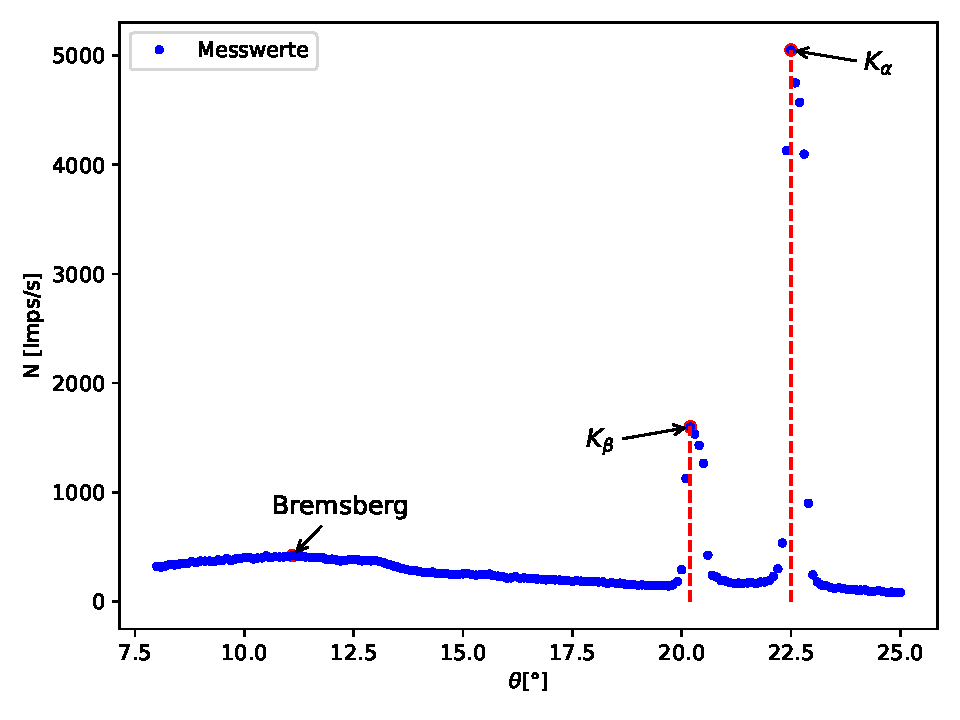
\includegraphics[scale = 0.9]{auswertung/plot1.pdf}
    \caption{$\theta-N$ Darstellung des Emissionsspektrums.}
    \label{fig:plot1}
\end{figure}
\noindent
Für die Spektrallinien wird nun die Wellenlänge $\lambda$ mittels Gleichung \eqref{eqn:(3)} berechnet und mit dem Zusammenhang
\eqref{eqn:E=hc/lambda} als Energie angegeben. Die Ergebnisse finden sich in Tabelle \ref{tab:energie}.
\begin{table}[H]
    \centering
        \caption{Photonenergie bei $K_{\alpha}$ und $K_{\beta}$}
        \label{tab:energie}
        \sisetup{table-format=4.1}
        \begin{tabular}{S S S S}
          \toprule
          {Spektrallinie} & {Energie $[\si{\kilo\electronvolt}]$} & {Literaturwert \cite{AP03} $[\si{\kilo\electronvolt}]$} & {Abweichung [\%]}\\
          \midrule
          {$K_{\alpha}$} & 8.044 & 8.048 & 0.0472 \\
          {$K_{\beta} $} & 8.915 & 8.907 & -0.091 \\
          \bottomrule
        \end{tabular}
      \end{table}

\subsection{Bestimmung der Transmission als Funktion der Wellenlänge}
\label{sec:transmission}
Um die Transmission $T$ zu errechnen werden nach Gleichung \eqref{eqn:trans} $I_{0}$ und $I_{Al}$ benötigt. Diese werden aus den Messdaten
aus Tabelle \ref{tab:mess2} mittels Gleichung \eqref{eqn:(4)} berechnet. Die so gewonnene Transmission wurde dann mittels 
\textit{matplotlib} \cite{matplotlib} in einem $\lambda-T$ Diagramm in Abbildung \ref{fig:plot2} aufgetragen. Dabei ist die Wellenlänge
$lambda$ zuvor wieder mit mittels Gleichung \eqref{eqn:(3)} berechnet worden. Die angegebenen Fehlerbalken beruhen auf der Poisson-Verteilung
$\Delta N=\sqrt{N}$.
\begin{figure}[H]
    \centering
    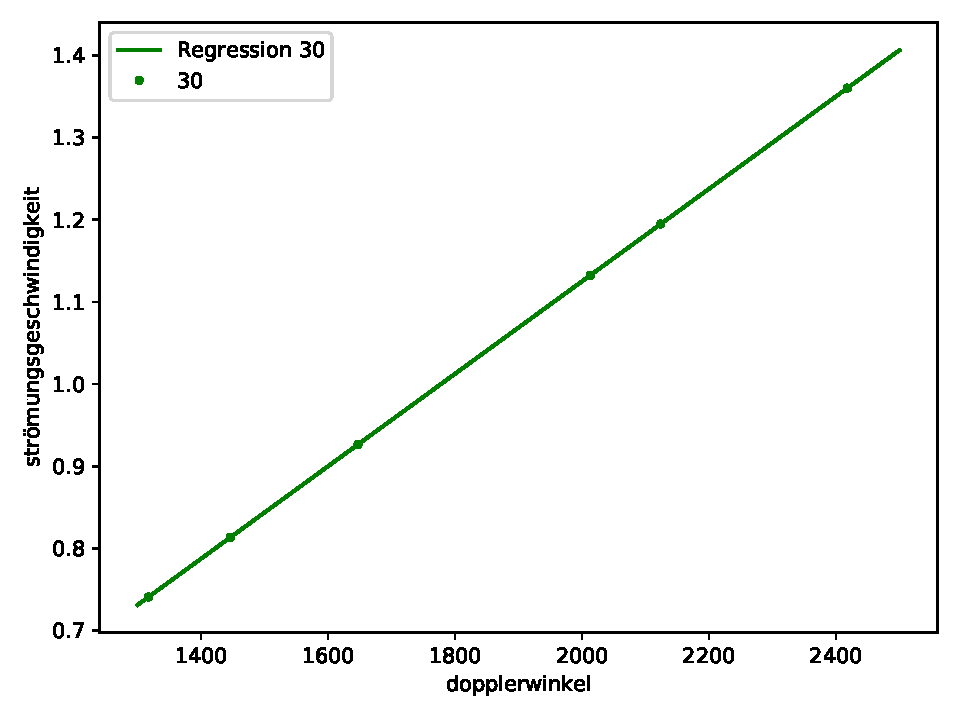
\includegraphics[scale = 0.9]{auswertung/plot2.pdf}
    \caption{Die Transmission in Abhängingkeit der Wellenlänge.}
    \label{fig:plot1}
\end{figure}
\noindent
Die eingezeichnete Regression hat dabei eine Funktionsgleichung der Form
  \begin{equation*}
      y=a\cdot x+b \label{eqn:gerade}
  \end{equation*} 
mit
  \begin{align*}
    a &= \SI{-0.015 \pm 0.000}{\per\pico\metre}\\
    b &= \SI{1.225 \pm 0.014}.
  \end{align*}
Die Unsicherheiten wurden dabei von  \textit{numpy} \cite{numpy} berechnet.

\subsection{Bestimmung der Compton-Wellenlänge}
\label{sec:compton}
Für die Bestimmung der Compton-Wellenlänge $\lambda_c$ werden nach \ref{sec:diskussion3} $I_0$, $I_1$ und $I_2$ benötigt.
Die Messung ergab
\begin{align*}
    I_0 &= 2731 \si{Imp}\\
    I_1 &= 1180 \si{Imp}\\
    I_2 &= 1024 \si{Imp}.
\end{align*}  
Durch diese werden die Transmissionen $T_1=I_1/I_0$ und  $T_2=I_2/I_0$ berechnet, womit sich dann die Wellenlänge durch Gleichung
\eqref{eqn:lambda} berechnen lässt. Dafür werden die Parameter der linearen Regression verwendet, also wird \eqref{eqn:lambda} zu
\begin{equation*}
    \lambda_i = \frac{T_i -b}{a}. 
\end{equation*}
Einsetzen der berechneten Werte ergibt dann
\begin{align*}
    \lambda_1 &= \SI{52.189}{\pico\metre}\\
    \lambda_2 &= \SI{55.948}{\pico\metre}.
\end{align*}
Somit ist die berechnete Compton-Wellenlänge
\begin{equation*}
    \lambda_c=\lambda_2-\lambda_1= \SI{3.7593}{\pico\metre}.
\end{equation*}